\chapter{Los metales: reacciones con los ácidos y corrosión}\label{ch:g9:metals-acids-corrosion}

En un puerto, el casco de acero de un viejo pesquero está surcado de
regueros anaranjados de \omterm{def:g9:metals-acids-corrosion:corrosion}{herrumbre}. En el muelle, una verja recubierta de
cinc lleva treinta años bajo la lluvia y sigue teniendo un brillo gris
apagado. En un museo, un anillo de oro enterrado durante tres mil años
brilla como el día en que se hizo. Los metales no se enfrentan al mundo
todos de la misma manera: a unos los atacan el agua, el \omterm{def:g4:air-a-mixture-of-gases:air}{aire} y los
ácidos, y a otros apenas.

\begin{recall}
Los \omterm{def:g9:ions:ion}{iones} son \omterm{def:g7:atoms-and-molecules:atom}{átomos} con carga; los metales dan \omterm{def:g9:ions:ion}{cationes} como
\ce{Fe^{2+}}, \ce{Zn^{2+}}, \ce{Al^{3+}}, que se identifican mediante
ensayos de \omterm{def:g9:ions:precipitate}{precipitación} (\cref{ch:g9:ions}). Una \omterm{def:g9:acids-bases-ph:acidic}{disolución ácida}
contiene muchos \omterm{def:g9:ions:ion}{iones} \ce{H+(aq)} (\cref{ch:g9:acids-bases-ph}). El
hidrógeno \omterm{def:g4:what-a-fire-needs:burning}{arde} con un pop agudo en la boca de un tubo de ensayo
(\cref{ch:g7:identifying-substances}).
\end{recall}

\begin{omfigure}
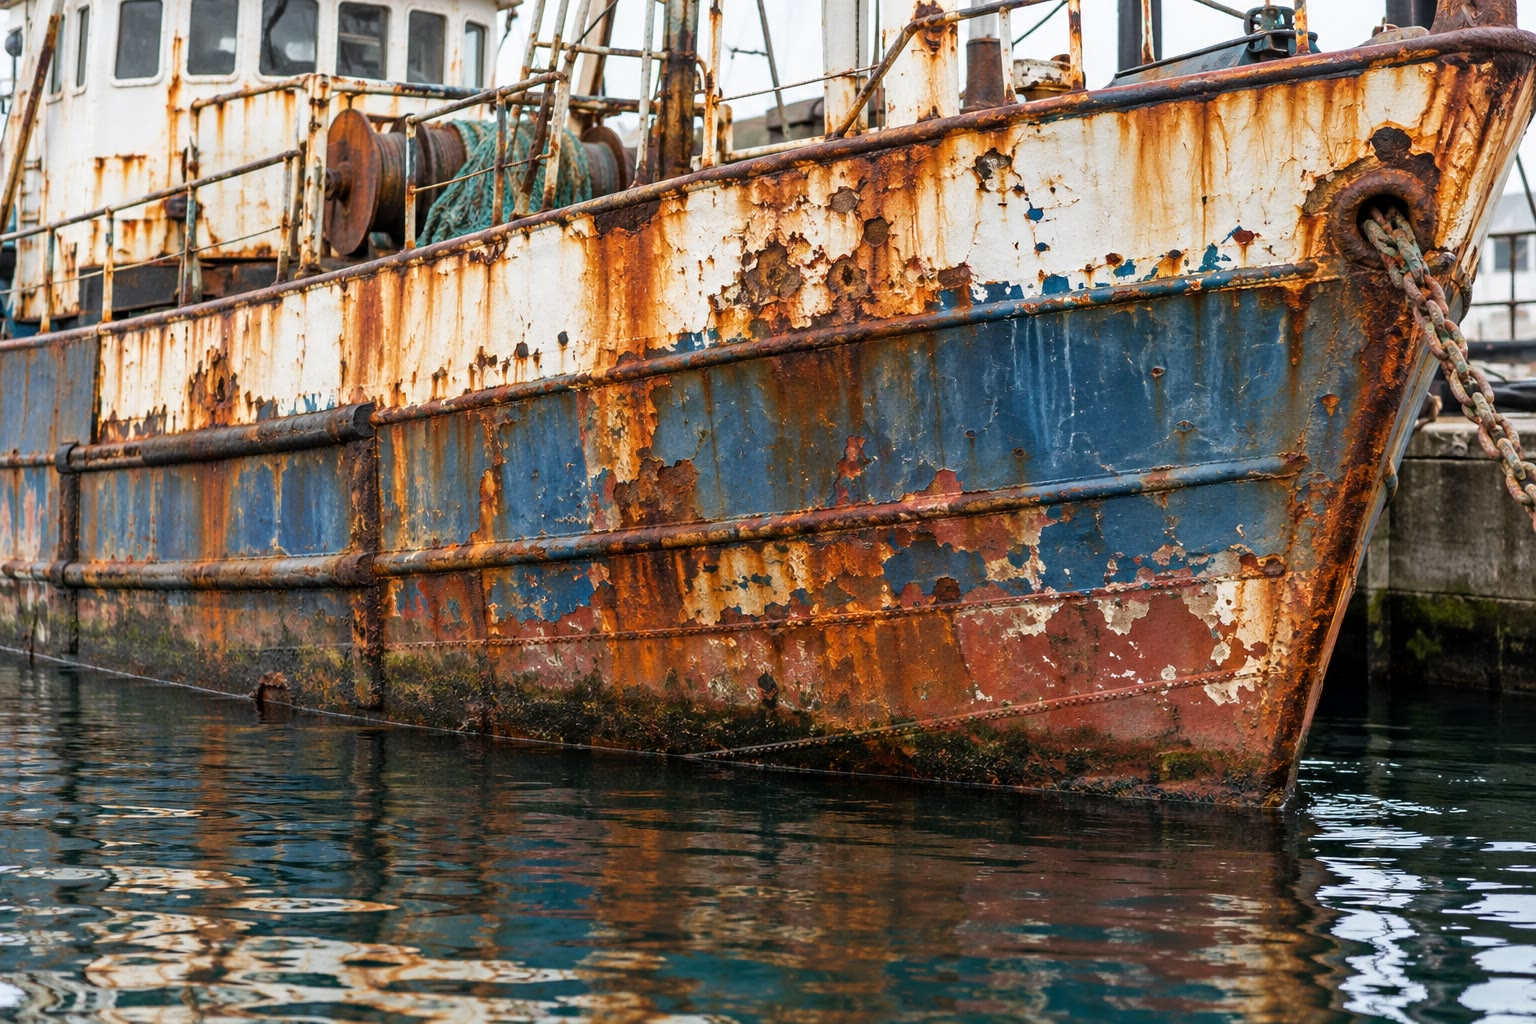
\includegraphics[width=0.55\linewidth]{images/book1/ai/g9-rusty-hull.jpg}

{\small El casco de un barco viejo: el acero se está oxidando.}
\end{omfigure}

\section{Los metales en ácido clorhídrico}

\begin{inthelab}[Tres metales en ácido]
El profesor echa un trocito de hierro, uno de cinc y uno de cobre en
tres tubos de ensayo con ácido clorhídrico diluido. Del hierro y del
cinc suben burbujas, despacio del hierro y con viveza del cinc, y los
metales van desapareciendo poco a poco; al cobre no le pasa nada. El
gas, recogido en un tubo pequeño, da un pop agudo: es hidrógeno. Con
hidróxido de sodio, el líquido del primer tubo da un \omterm{def:g9:ions:precipitate}{precipitado} verde
(\omterm{def:g9:ions:ion}{iones} \ce{Fe^{2+}}), y el del segundo, uno blanco (\omterm{def:g9:ions:ion}{iones} \ce{Zn^{2+}}).
\end{inthelab}

\begin{omfigure}
\begin{tikzpicture}[font=\small, scale=1.2]
  \foreach \k/\m/\c/\bub in {0/hierro/black!45/4, 1/cinc/black!25/9, 2/cobre/orange!60!brown/0} {
    \pic[transform shape] at (\k*2.4,0) {testtube={0.55}{omWater!70}};
    \fill[\c] (\k*2.4-0.13,0.08) rectangle (\k*2.4+0.13,0.35);
    \ifnum\bub>0
      \foreach \j in {1,...,\bub} {
        \pgfmathsetmacro\yy{0.45+0.12*\j}
        \pgfmathsetmacro\xx{\k*2.4+0.1*sin(97*\j)}
        \draw[black!55] (\xx,\yy) circle (0.035);
      }
    \fi
    \node[anchor=north, align=center] at (\k*2.4,-0.15) {\m};
  }
  \node[anchor=north, align=center, font=\footnotesize] at (0,-0.6) {burbujeo lento};
  \node[anchor=north, align=center, font=\footnotesize] at (2.4,-0.6) {burbujeo vivo};
  \node[anchor=north, align=center, font=\footnotesize] at (4.8,-0.6) {no reacciona};
\end{tikzpicture}

{\small Hierro, cinc y cobre en ácido clorhídrico diluido: el hierro y el
cinc desprenden hidrógeno; el cobre no reacciona.}
\end{omfigure}

\begin{proposition}[Metal más ácido]\label{prop:g9:metals-acids-corrosion:acid}
Muchos metales (el hierro, el cinc, el aluminio, el magnesio) reaccionan
con los \omterm{def:g9:ions:ion}{iones} \ce{H+} de un ácido: el metal desaparece en forma de \omterm{def:g9:ions:ion}{iones}
metálicos, que quedan disueltos, y se desprende hidrógeno gaseoso. El
cobre, la plata y el oro no reaccionan con el ácido clorhídrico.
\end{proposition}

\section{Escribir la ecuación con iones}

\begin{definition}[Ion espectador]\label{def:g9:metals-acids-corrosion:spectator}
Un \omterm{def:g9:ions:ion}{ion} que está presente en una disolución durante una reacción pero no
interviene en ella, y que se encuentra sin cambios al final, es un
\emph{ion espectador}\index{ion espectador}. Se omite en la ecuación.
\end{definition}

\begin{example}[El hierro y el cinc en ácido clorhídrico]\label{ex:g9:metals-acids-corrosion:iron}
El ácido clorhídrico contiene \omterm{def:g9:ions:ion}{iones} \ce{H+(aq)} y \ce{Cl-(aq)}. Los
\omterm{def:g9:ions:ion}{iones} cloruro se encuentran sin cambios al final: son espectadores. Las
ecuaciones son
\[
  \ce{Fe(s) + 2H+(aq) -> Fe^{2+}(aq) + H2(g)}, \qquad
  \ce{Zn(s) + 2H+(aq) -> Zn^{2+}(aq) + H2(g)}.
\]
Están ajustadas tanto en \omterm{def:g7:atoms-and-molecules:atom}{átomos} como en cargas: $+2$ en cada miembro.
\end{example}

\begin{method}[Escribir la ecuación de un metal con un ácido]\label{met:g9:metals-acids-corrosion:write}
\begin{enumerate}
  \item \omterm{def:g7:chemical-reactions:reactant}{Reactivos}: el metal (s) y los \omterm{def:g9:ions:ion}{iones} \ce{H+(aq)}.
  \item Productos: el \omterm{def:g9:ions:ion}{ion} metálico (aq), con su carga habitual, y el
        hidrógeno \ce{H2(g)}.
  \item Ajustar los \omterm{def:g7:atoms-and-molecules:atom}{átomos} y comprobar después que la carga total es la
        misma en los dos miembros.
\end{enumerate}
Para el aluminio: \ce{2Al(s) + 6H+(aq) -> 2Al^{3+}(aq) + 3H2(g)}; carga
$+6$ en cada miembro.
\end{method}

\begin{safety}{\ghs[0.8cm]{GHS02}\ghs[0.8cm]{GHS04}}
% ledger: ghs:H2
El hidrógeno que se desprende es extremadamente inflamable. La reacción
la hace el profesor en tubos de ensayo pequeños, lejos de cualquier
llama salvo la que se usa para el ensayo del pop.
\end{safety}

\section{La corrosión}

\begin{definition}[Corrosión y herrumbre]\label{def:g9:metals-acids-corrosion:corrosion}
La \emph{corrosión}\index{corrosion@corrosión} es el ataque lento de un metal por
las sustancias que lo rodean (el oxígeno, el agua, los ácidos, las
sales), que convierte el metal en \omterm{def:g9:ions:ion}{iones} o en compuestos como los
óxidos. La corrosión del hierro y del acero produce
\emph{herrumbre}\index{herrumbre}, un óxido de hierro hidratado, pardo y
quebradizo, que se desprende en escamas y deja que el ataque siga más
adentro.
\end{definition}

\begin{proposition}[Lo que necesita el hierro para oxidarse]\label{prop:g9:metals-acids-corrosion:needs}
El hierro solo se oxida cuando le llegan a la vez el oxígeno y el agua.
La sal disuelta en el agua, como en las carreteras a las que se echa
sal en invierno o junto al mar, acelera la oxidación.
\end{proposition}

\begin{inthelab}[Tres clavos, una semana]
Se colocan tres clavos de hierro limpios en tres tubos de ensayo: el
primero con \omterm{def:g4:air-a-mixture-of-gases:air}{aire} seco y un desecante que elimina el vapor de agua; el
segundo en agua hervida para eliminar el \omterm{def:g4:air-a-mixture-of-gases:air}{aire} disuelto, cubierta con una
capa de aceite; el tercero, mitad en agua del grifo y mitad en el \omterm{def:g4:air-a-mixture-of-gases:air}{aire}.
Al cabo de una semana, solo el tercer clavo está oxidado.
\end{inthelab}

\begin{omfigure}
\begin{tikzpicture}[font=\small, scale=1.2]
  % tube 1: dry air, drying agent
  \pic[transform shape] at (0,0) {testtube={0.18}{white!80!black}};
  \foreach \x/\y in {-0.12/0.15,0.08/0.12,-0.02/0.3,0.12/0.32,-0.14/0.42,0.03/0.48}
    \fill[black!35] (\x,\y) circle (0.05);
  \fill[black!45] (-0.03,1.0) rectangle (0.03,2.4);
  \fill[black!45] (-0.09,2.4) rectangle (0.09,2.48);
  \fill[black!60] (-0.3,2.8) rectangle (0.3,3.1);
  \node[anchor=north, align=center] at (0,-0.15) {aire seco:\\ sin herrumbre};
  % tube 2: boiled water under oil
  \pic[transform shape] at (2.6,0) {testtube={0.7}{omWater!80}};
  \fill[yellow!55!orange!60] (2.36,1.85) rectangle (2.84,2.1);
  \fill[black!45] (2.57,0.3) rectangle (2.63,1.7);
  \fill[black!45] (2.51,1.7) rectangle (2.69,1.78);
  \fill[black!60] (2.3,2.8) rectangle (2.9,3.1);
  \node[anchor=north, align=center] at (2.6,-0.15) {agua sin aire:\\ sin herrumbre};
  % tube 3: water and air
  \pic[transform shape] at (5.2,0) {testtube={0.4}{omWater!80}};
  \fill[black!45] (5.17,0.3) rectangle (5.23,2.2);
  \fill[black!45] (5.11,2.2) rectangle (5.29,2.28);
  \fill[orange!60!brown] (5.15,0.9) rectangle (5.25,1.5);
  \node[anchor=north, align=center] at (5.2,-0.15) {agua y aire:\\ herrumbre};
  \draw[<-, omProp, thick] (-0.15,0.3) -- (-0.9,0.7) node[left, text=black, font=\footnotesize] {desecante};
  \draw[<-, omProp, thick] (2.85,1.98) -- (3.6,2.4) node[right, text=black, font=\footnotesize] {aceite};
\end{tikzpicture}

{\small El experimento de los tres clavos: el hierro solo se oxida donde
le llegan juntos el agua y el oxígeno, aquí en la superficie del agua.}
\end{omfigure}

\begin{example}[El aluminio y el cobre se protegen solos]\label{ex:g9:metals-acids-corrosion:protect}
El oxígeno del \omterm{def:g4:air-a-mixture-of-gases:air}{aire} ataca enseguida el aluminio, pero la fina capa de
óxido que se forma se adhiere al metal y lo aísla del \omterm{def:g4:air-a-mixture-of-gases:air}{aire}: las
ventanas de aluminio duran décadas. El cobre, atacado lentamente por el
\omterm{def:g4:air-a-mixture-of-gases:air}{aire}, el agua y el dióxido de carbono, se cubre de una costra verde, la
pátina, que también se adhiere y protege el metal de debajo. La
\omterm{def:g9:metals-acids-corrosion:corrosion}{herrumbre}, en cambio, se desprende en escamas.
\end{example}

\begin{omfigure}
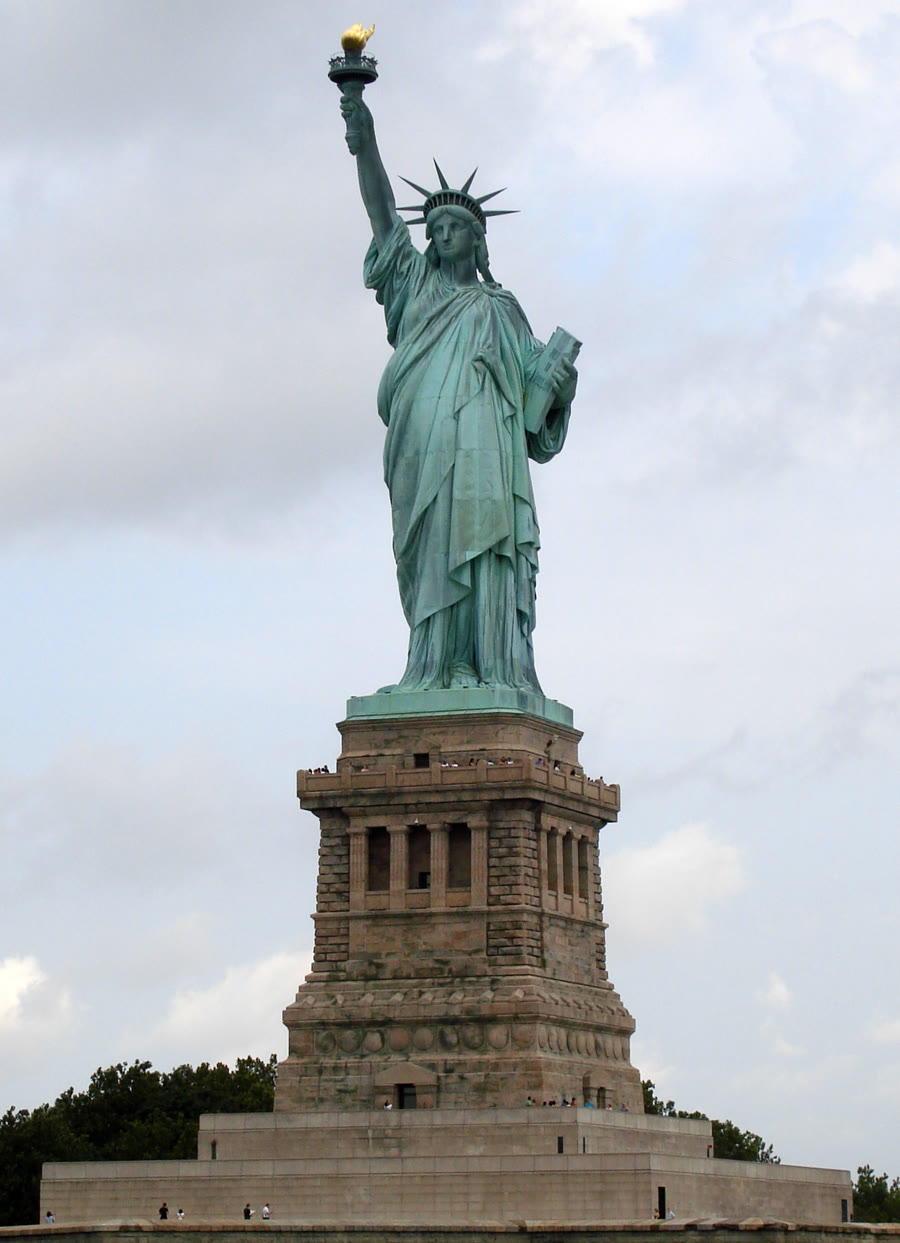
\includegraphics[height=6cm]{images/book1/statue-patina.jpg}

{\small La estatua de la Libertad: su piel de cobre está cubierta de una
pátina verde. Foto: Elcobbola, dominio público.}
\end{omfigure}

\section{Proteger los metales}

\begin{definition}[Galvanizado]\label{def:g9:metals-acids-corrosion:galvanising}
El \emph{galvanizado}\index{galvanizado} consiste en recubrir el acero
con una capa de cinc, sumergiéndolo en cinc fundido. El \omterm{def:g4:air-a-mixture-of-gases:air}{aire} y el agua
atacan el cinc en lugar del acero de debajo: incluso donde el
recubrimiento está rayado, el cinc cercano se corroe primero y el acero
se libra.
\end{definition}

\begin{proposition}[Formas de proteger el hierro y el acero]\label{prop:g9:metals-acids-corrosion:ways}
\begin{itemize}
  \item mantener lejos el agua y el \omterm{def:g4:air-a-mixture-of-gases:air}{aire}: pintura, aceite, grasa, un
        recubrimiento de \omterm{def:g8:plastics:plastic}{plástico};
  \item galvanizar: una capa de cinc que se corroe en lugar del acero;
  \item usar acero inoxidable, una aleación de hierro con cromo, que se
        protege a sí misma con una fina capa de óxido aislante;
  \item fijar bloques de cinc a los cascos de los barcos: el cinc se va
        consumiendo poco a poco en lugar del acero y se sustituye de vez
        en cuando (cómo funciona se explica en un volumen universitario).
\end{itemize}
\end{proposition}

\begin{omfigure}
\begin{minipage}[b]{0.52\linewidth}\centering
\begin{tikzpicture}[font=\small]
  \fill[black!35] (0,0) rectangle (5,0.8);
  \fill[black!15] (0,0.8) rectangle (2.2,1.1);
  \fill[black!15] (2.8,0.8) rectangle (5,1.1);
  \fill[omWater!80] (1.6,1.1) rectangle (3.4,1.35);
  \fill[omWater!80] (2.2,0.8) rectangle (2.8,1.1);
  \draw[black!60] (0,0) rectangle (5,0.8);
  \foreach \x in {1.95,2.1} \draw[->, omProp, thick] (\x,1.25) -- (\x+0.05,1.7);
  \node[anchor=west, font=\footnotesize] at (5.1,0.4) {acero};
  \node[anchor=west, font=\footnotesize] at (5.1,0.95) {capa de cinc};
  \node[anchor=south, font=\footnotesize, align=center] at (2.0,1.75) {los iones cinc\\ pasan al agua};
  \node[anchor=north, font=\footnotesize, align=center] at (2.5,-0.05) {una raya: el acero\\ queda al descubierto, pero\\ el cinc de alrededor se corroe antes};
\end{tikzpicture}

{\small Una chapa galvanizada rayada.}
\end{minipage}\hfill
\begin{minipage}[b]{0.44\linewidth}\centering
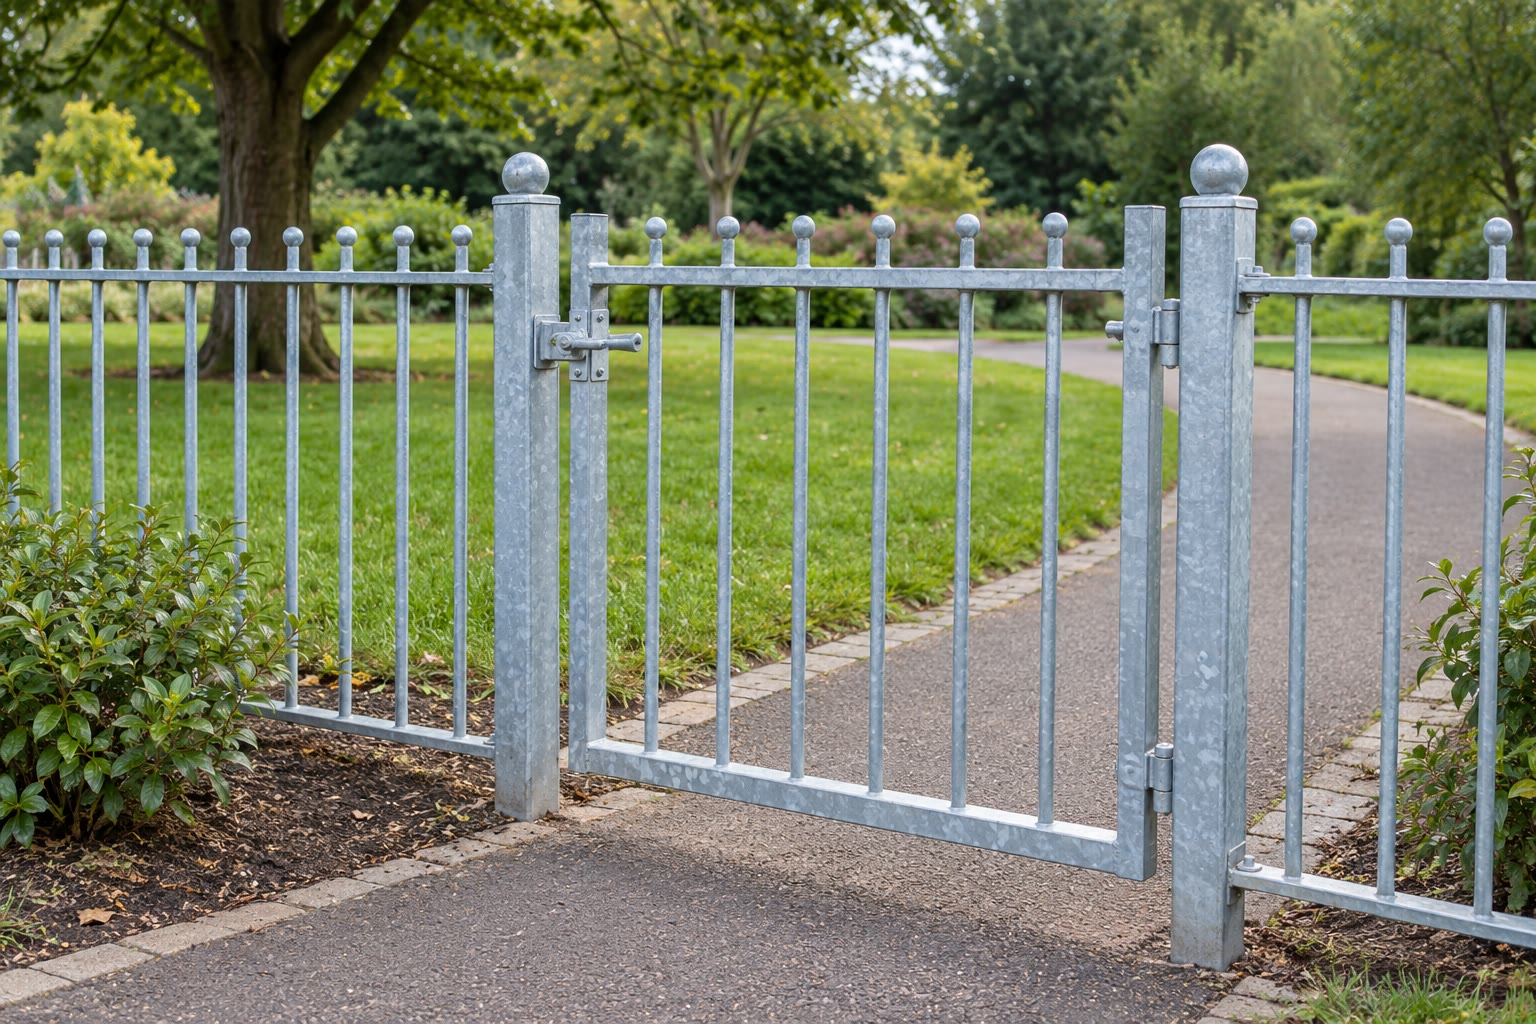
\includegraphics[width=\linewidth,height=4.4cm,keepaspectratio]{images/book1/ai/g9-galvanised-railings.jpg}

{\small Una barandilla de acero \omterm{def:g9:metals-acids-corrosion:galvanising}{galvanizado}.}
\end{minipage}
\end{omfigure}

\section{Ejercicios}

\begin{exercise}[$\star$]\label{exo:g9:metals-acids-corrosion:1}
¿Qué gas se desprende cuando el cinc reacciona con el ácido clorhídrico?
¿Cómo se identifica?
\end{exercise}

\begin{exercise}[$\star$]\label{exo:g9:metals-acids-corrosion:2}
¿Cuáles de estos metales reaccionan con el ácido clorhídrico diluido: el
hierro, el cobre, el cinc, el oro, el aluminio?
\end{exercise}

\begin{exercise}[$\star$]\label{exo:g9:metals-acids-corrosion:3}
¿Qué necesita el hierro para oxidarse?
\end{exercise}

\begin{exercise}[$\star$]\label{exo:g9:metals-acids-corrosion:4}
¿Qué es un \omterm{def:g9:metals-acids-corrosion:spectator}{ion espectador}? Nombra el \omterm{def:g9:metals-acids-corrosion:spectator}{ion espectador} cuando el hierro
reacciona con el ácido clorhídrico.
\end{exercise}

\begin{exercise}[$\star\star$]\label{exo:g9:metals-acids-corrosion:5}
Escribe la ecuación de la reacción del magnesio con los \omterm{def:g9:ions:ion}{iones} \ce{H+} de
un ácido (el \omterm{def:g9:ions:ion}{ion} magnesio es \ce{Mg^{2+}}). Comprueba las cargas.
\end{exercise}

\begin{exercise}[$\star\star$]\label{exo:g9:metals-acids-corrosion:6}
Después de que el hierro haya reaccionado con el ácido clorhídrico,
¿cómo puedes mostrar que la disolución contiene \omterm{def:g9:ions:ion}{iones} hierro(II)?
\end{exercise}

\begin{exercise}[$\star\star$]\label{exo:g9:metals-acids-corrosion:7}
Mira la figura de los tres clavos. ¿Por qué el agua del segundo tubo se
ha hervido y se ha cubierto con aceite?
\end{exercise}

\begin{exercise}[$\star\star$]\label{exo:g9:metals-acids-corrosion:8}
¿Por qué un coche se oxida más deprisa en una ciudad donde se echa sal
en las calles en invierno?
\end{exercise}

\begin{exercise}[$\star\star$]\label{exo:g9:metals-acids-corrosion:9}
¿Por qué las ventanas de aluminio no se corroen hasta desaparecer,
aunque el aluminio reaccione con el oxígeno del \omterm{def:g4:air-a-mixture-of-gases:air}{aire}?
\end{exercise}

\begin{exercise}[$\star\star$]\label{exo:g9:metals-acids-corrosion:10}
Da tres maneras de proteger de la \omterm{def:g9:metals-acids-corrosion:corrosion}{herrumbre} el cuadro de acero de una
bicicleta.
\end{exercise}

\begin{exercise}[$\star\star\star$]\label{exo:g9:metals-acids-corrosion:11}
Escribe y comprueba la ecuación de la reacción del aluminio con los
\omterm{def:g9:ions:ion}{iones} \ce{H+} de un ácido. ¿Cuántas \omterm{def:g7:atoms-and-molecules:molecule}{moléculas} de hidrógeno se forman por
cada 200 \omterm{def:g7:atoms-and-molecules:atom}{átomos} de aluminio?
\end{exercise}

\begin{exercise}[$\star\star\star$]\label{exo:g9:metals-acids-corrosion:12}
Un cubo de acero \omterm{def:g9:metals-acids-corrosion:galvanising}{galvanizado} tiene una raya que llega hasta el acero.
Explica por qué el acero del fondo de la raya tarda mucho en oxidarse.
\end{exercise}

\section{Problema: ¿Qué espesor tiene el cinc?}

\begin{problem}[{Problema de fin de semana --- disolver el
recubrimiento de cinc de una chapa galvanizada para averiguar qué
espesor tenía}]
\label{pb:g9:metals-acids-corrosion:1}
% ledger: rho:Zn
Una chapa de acero \omterm{def:g9:metals-acids-corrosion:galvanising}{galvanizado}, un cuadrado de \qty{10.0}{cm} de lado,
está recubierta de cinc por las dos caras (se desprecian los bordes). En
un laboratorio, el profesor la pesa, \qty{125.6}{g}, y luego la sumerge
en ácido clorhídrico que contiene un aditivo que impide que el ácido
ataque el acero. Cuando deja de burbujear, la chapa se enjuaga, se seca
y se vuelve a pesar: \qty{113.5}{g}. La masa de \qty{1}{cm^3} de cinc es
\qty{7.13}{g}.

\medskip
\noindent\textbf{Parte I --- La reacción.}
\begin{enumerate}
  \item Escribe la ecuación de la reacción del cinc con los \omterm{def:g9:ions:ion}{iones}
        \ce{H+} del ácido.
  \item ¿Qué gas produce el burbujeo? Describe su ensayo.
  \item ¿Qué ensayo mostraría después los \omterm{def:g9:ions:ion}{iones} cinc en la disolución?
  \item Nombra los \omterm{def:g9:metals-acids-corrosion:spectator}{iones espectadores}.
\end{enumerate}

\medskip
\noindent\textbf{Parte II --- El cinc.}
\begin{enumerate}[resume]
  \item ¿Qué masa de cinc se ha disuelto?
  \item ¿Por qué el burbujeo indica que todavía no se ha disuelto todo
        el cinc?
  \item ¿Qué le pasaría al acero si el ácido no contuviera el aditivo?
        ¿Qué ensayo lo mostraría entonces?
  \item ¿Por qué el cinc protege el acero de la chapa mientras sigue
        ahí?
\end{enumerate}

\medskip
\noindent\textbf{Parte III --- El espesor.}
\begin{enumerate}[resume]
  \item ¿Cuál es la superficie total recubierta de la chapa, en
        \unit{cm^2}?
  \item ¿Qué volumen ocupaba el cinc?
  \item Deduce el espesor de la capa de cinc, en centímetros.
  \item Expresa ese espesor en micrómetros
        (\qty{1}{cm} $= \qty{10000}{\micro m}$).
\end{enumerate}
\end{problem}
